\chapter{Knowledge Discovery and Data Mining}\label{chapter:kdd}
In this chapter we clarify the terms and the importance of knowledge discovery and data mining. In a nutshell it is the process of discovering knowledge and patterns from data. Therefore, many tools and algorithms exist which we describe in the following sections.
\section{Motivation}
As already mentioned, data growth is exploding and new data is generated every day by every aspect of daily life, such as businesses, society, science and medicine. With this huge amount of data available, it has become one of the most valuable resources of our decade. News and Blogs are even considering data as important as oil\footnote{http://www.forbes.com/sites/perryrotella/2012/04/02/is-data-the-new-oil/.} or as the new currency of our decade\footnote{http://www.europeanvoice.com/event/data-the-new-currency/.}. 
\\
However, before data has any value it has to be transformed into knowledge. For example, e-commerce companies are very keen to find out not only what their customers have bought but also what they are likely to buy in the future. This knowledge is then used to generate more revenue. A very well known example is amazon.com which is advertising a variety of similar products the customer recently looked for, or products another customer with similar characteristics has purchased in the past. Therefore data mining techniques are used to boost consumerism. Additionally, this knowledge might be used to optimize storage cost, e.g. by knowing how much of certain products will be needed to distribute in the next weeks.
\\
Other areas for data mining are telecommunication network carriers with a huge amount of data traffic generated every day, the health and medical industry and the Web in general, to name just a few examples. Again it is all about knowledge. The telecommunication network carriers are interested in customer usage behaviour, while state authorities are interested in wiretapping of potential criminals. Medical data might be used to install an ameliorated patient monitoring and Web data can be used for search engines to find the best results or for ad networks to deliver promising ads. The list of sources to generate data from and the knowledge one is interested in is endless.


\section{Knowledge Discovery}

After understanding the importance of data mining for gaining knowledge and using this knowledge for further decision making, this section defines data mining in greater detail. The term data mining itself often leads to confusion - we are not mining data but instead we are looking for knowledge and interesting patterns in a given data set or database. Therefore, the term knowledge discovery is often more appropriate.
\\
However, the usage of knowledge discovery and data mining as synonyms is not entirely accurate. Instead, data mining is often seen as a part of the knowledge discovery process as depicted in~\autoref{fig:kdd}. This process starts with the preprocessing steps data cleaning, integration, selection and transformation. Afterwards, data mining and its algorithms are applied and the discovered patterns are evaluated and presented. 
\\
In this work we use the term data mining as described in ~\autoref{fig:kdd} since we are mainly interested in the algorithms applied in the data mining phase. Nevertheless, future work on HyPer will cover the entire knowledge discovery chain and implement techniques to clean the data as well to present the results. Therefore, this section gives a profound overview over all the knowledge discovery steps; a focus on the data mining algorithms follows in Section~\ref{section:datamining}.


\begin{figure}[htsb]
  \centerline{
    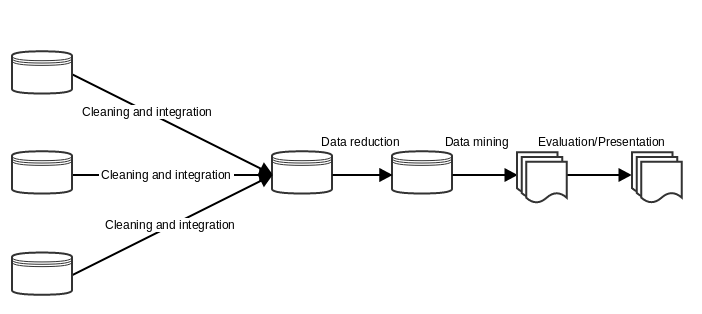
\includegraphics[scale=0.6]{figures/kdd}
  }
  \caption[The Process of Knowledge Discovery]{The Process of Knowledge Discovery.}\label{fig:kdd}
\end{figure}


Regarding all those steps, Han et al.~\parencite[8]{dmbook} give a detailed definition of data mining: 
\begin{quote}
“Data mining is the process of discovering interesting patterns and knowledge from large amounts of data. The data sources can include databases, data warehouses, the Web, other information repositories, or data that are streamed into the system dynamically.”
\end{quote}

In the following sections we discuss each phase in detail and start with data cleaning. 

\subsection{Data Cleaning} 
The first step of knowledge discovery needs to ensure that the data we are interested in is complete, clean and consistent. Real world data is usually none of it. Data sets are incomplete, i.e. values are missing. If these missing values are crucial for the further data mining process, several data cleaning techniques exist to fill the gaps, e.g. by using an average value such as the mean or the median.
\\
The same is true for inconsistent or redundant data. An example of inconsistent data are distinct values with the same meaning. Additionally, we often see random error or variance in a measured variable. This is called noisy data and must be cleaned for proper data analysis e.g. by smoothing the data set, using binning techniques.


\subsection{Data Integration}

Data mining often requires data from several sources. These sources can be databases, data warehouses, transactional data or plain data files. Also complex data might be used, such as time-related data, data streams, spatial data, multimedia data and graph data. All of these sources have to be integrated into one coherent data set which is then used for further analysis. There are several challenges regarding data integration, the most important is the entity identification problem: When combining data from different sources same data objects can have different names and types in different schemas. Therefore, data integration often requires domain knowledge of the different data sources and techniques used in the data cleaning phase to get a clean, consistent data set and to avoid redundancy.


\subsection{Data Reduction}

After cleaning and integrating data into a coherent data set, the data is ready for further mining. However, those data sets are often of huge size and contain much information, not all necessary for the data mining process. Data reduction techniques can help to reduce the information density and speed up the data analysis and mining process. Simple techniques for data reduction are projection, selection and aggregation, available in every database system. More advanced techniques are dimensionality reduction, e.g. by a principal component analysis, numerosity reduction above aggregation, e.g. clustering or sampling, and data compression. 
\\
Other methods are data transformations which change the data by converting values into another format e.g. by using normalization. Another possibility is data discretization, e.g. by transforming numeric data into intervals. 
\\
The aim of all of the addressed methods is to reduce the size of the initial data set and therefore to make it easier to get the information the user is interested in. Some methods of the presented data reduction techniques are data mining techniques as well, e.g. clustering. Therefore the boundary between data reduction and data mining is not always easy to set.


\subsection{Data Mining}

After applying the presented preprocessing steps the data set is now ready for data mining techniques. In the data mining phase we apply algorithms for finding interesting patterns in the data set. Crucial techniques are mining frequent patterns and association rules, classification, clustering and outlier detection. Algorithms for performing those techniques are presented in Section ~\ref{section:datamining}. 


\subsection{Pattern Evaluation}

After generating those patterns we have to evaluate them to figure out how valuable the acquired knowledge is. There exist several criteria for pattern evaluation. First, a pattern has to be understandable. A clustering for example does not give any knowledge if the reason for the clustering is not comprehensible. Therefore, the reasons of a data mining pattern must be clear for the user. That leads to the next criteria of evaluation: A pattern has to be valid, useful and novel. Only then, a pattern can be called interesting and can be used as knowledge, e.g. by fulfilling a hypothesis the user tries to confirm. 


\subsection{Knowledge Presentation}

Knowledge presentation is the final step of knowledge discovery. Interesting patterns have to be described and visualized to the user in an appealing, understandable format. Apart from textual explanation, several data visualization techniques exist and should be applied for the respective situation.


\section{Algorithms of Data Mining}\label{section:datamining}
In the following sections we discuss data mining techniques such as frequent itemset mining, classification, clustering and outlier detection.
For each group the purpose of the technique is given and its most important algorithms are presented.

\subsection{Mining Frequent Patterns and Association Rules}
Frequent pattern mining aims to find the most frequent items in a data set and its association rules. A typical example is the market basket analysis: Supermarkets and e-commerce stores are interested in what their customers are buying, in particular in items that are commonly bought together. In other words, which items are frequently put in the same market basket?
\\
This knowledge is very valuable: It is not only about finding out which items are very popular and therefore get a better a position in the market or website. It is also about knowing which items are bought together which can lead to interesting desicions: Related items could be placed next to each other to make the shopping experience for the customer more convenient. Another approach could be to put related items far away from each other, so that the customer has to walk around in the store and is more likely to buy an additional product. These are just two possible strategies that could be applied with the knowledge resulting from frequent pattern mining.
\\
Most algorithms for frequent pattern mining expect transactional data as input, because this type of data represents a market basket the best. The most popular algorithm is the Apriori algorithm~\parencite{apriori}, working in an iterative manner. Apriori generates itemsets of length $k$ and checks if these itemsets appear frequently, i.e. if their count exceeds a given threshold. All the valid itemsets are then used in the next iteration to generate itemsets of length $k+1$. The algorithm converges if no more itemsets can be generated.
\\
Since the candidate generation and the scanning of the database is expensive, there are attempts to improve the Apriori performance, e.g.~\parencite{ap1}\parencite{ap2} as well as to establish other techniques. One of them is Frequent-Pattern-growth (FP-growth)~\parencite{fpgrowth}, an algorithm compressing the database into an FP-tree and therefore finding frequent itemsets without itemset generation. Furthermore, there exist algorithms for more specific cases, e.g. for finding frequent patterns in high-dimensional, spatial and multimedia data.

\subsection{Classification}

In data mining, classification uses existing data as knowledge for predicting future events. A typical example is the identification of spam emails. This is done by labeling existing emails and categorizing them as spam or non-spam. Such a data set is called the training data set. The algorithm uses then this training knowledge to classify new, unknown emails as spam or non-spam.
\\
Since classification needs training data it is also called~\emph{supervised learning}. That means that before the start of the data mining process, previous knowledge has to be acquired. In our example, someone has to label emails first as spam or non-spam before the algorithm can be applied. 
\\
There are many classification algorithms in practice, popular ones are Support Vector Machines (SVM)~\parencite{svm}, Decision Trees~\parencite{descisiontree} and Neural Networks~\parencite{neuralnetwork}.
\\
An SVM classifier starts by building a model upon a training data set. Each data tuple is represented as a vector in the SVM model space. Since the data is labeled the SVM knows which data tuples belong together and tries to find separating hyperplanes between them. These hyperplanes can be described by a small subset of the data vectors called the~\emph{support vectors}. This fact makes the SVM very efficient on high-dimensional data. Unknown data tuples are then modeled as a vector in the SVM space and belong to the same category as the other data tuples they are separated together with by the hyperplanes.

\subsection{Clustering}

While classification requires apriori knowledge, i.e. tuples must be labeled to be used as training data, clustering does not require any previous knowledge. In that sense, clustering is a very convenient method to gain knowledge about a data set without the need of knowing exactly what the result should look like. Therefore, clustering is also called~\emph{unsupervised learning}.
\\
An example is Google News, presenting and grouping news headlines obtained from many news websites. There is no predefined set of available news topics, instead the topics can change daily. Therefore, using classification with training data is not feasible. Instead, clustering can be used to find similar topics within the latest news articles and group them together. The clustering algorithm tries to find the best grouping of news, meaning that the news in one group have a high similarity with each other, while they are very different to the news in other groups. 
\\
Clustering techniques provide a variety of algorithms. These algorithms can be categorized in the following four groups:

\begin{itemize} 
\item Partitioning methods: Partitioning methods are the most popular clustering algorithms, trying to find clusters of spherical shape. A distance function is used to measure similarity and dissimilarity among the clusters. Popular algorithms are k-Means~\parencite{Lloyd82} and k-Medoids~\parencite{medoid}. 
\item Hierarchical methods: Hierarchical methods are useful for data consisting of several hierarchies or levels. Clustering is applied by going up or down the hierarchy tree by merging or splitting subtrees, respectively. Similar to partitioning-based methods, hierarchical cluster algorithms tend to find spherical clusters. 
\item Density-based methods: For finding clusters of arbitrary shape, such as oval or~\enquote{$S$-shaped} clusters, partitioning and hierarchical techniques are limited. Density-based clustering algorithms obtain much better results, using dense regions in data sets for identifying clusters instead of distances from a center point. The most popular algorithm is the DBSCAN (Density-based spatial clustering of Applications with Noise)~\parencite{dbscan} algorithm. It works by finding core objects, i.e. objects within a dense neighbourhood and joining those core objects together to find dense regions, i.e. clusters.
\item Grid-based methods: All the presented methods so far are data-driven, i.e. groupings are detected by the distribution of objects in the embedding space. In contrast, grid-based methods are space-driven, i.e. the object space is mapped to a finite number of cells, resulting in very fast processing times for multi-dimensional data. Popular algorithms are STING~\parencite{sting} and CLIQUE~\parencite{clique}. CLIQUE is a special form of a grid-based algorithm, since it is also density-based.
\end{itemize}





\subsection{Outlier Detection}

Outlier detection techniques aim to find data objects that behave in a different way than the majority of data objects. For an e-commerce system outliers can be clients spending much more money than the average client. This information is very valuable since the company is eager to make this client particularly happy, e.g. with special customer care treatment. Also in fraud detection and medical systems, outlier detection is very important to observe a security breach or a patient problem as early as possible.
\\
Obviously there is a strong correlation between outlier detection and clustering. Data objects that do not fit into a cluster are potential outliers. Therefore clustering techniques can be applied for outlier detection. However, their main purpose is to find clusters, whereas outlier detection algorithms are specialized in finding outliers. Often we have to optimize these algorithms to omit all dense areas to find outliers in a more efficient way.
\\
Apart from~\emph{unsupervised learning},~\emph{supervised learning} can be applied for outlier detection as well. First, data is labeled as normal or outlier, and upon that information future data can be classified. This data is then used as training data to classify data sets as outliers or normal data. The challenge of using classification methods for outlier detection is that outliers are very rare by definition, thus finding training instances resembling outliers is not trivial. Therefore typical classification algorithms often have to be adapted and optimized for outlier classification as well.
\\
Apart from clustering and classification techniques, statistical and proximity-based methods are also used for outlier detection.
\\
\\
The remainder of this work discusses and implements the clustering algorithm k-Means, one of the most well-known and popular data mining algorithm. It is implemented in most modern data mining tools such as R and Julia, and therefore a good comparison can be achieved. The algorithm is introduced in Chapter~\ref{chapter:kmeans} and implemented in Chapter~\ref{chapter:implementation}. The results are then discussed in Chapter~\ref{chapter:evaluation}.

